% CH 2 Hardware
\chapter{Yun-Trooper II硬體架構介紹}
\label{c:hardware}

\section{硬體架構簡介}
本論文之所開發的Yun-Trooper II是建置於TAMIYA公司的1:10四驅越野模型車TXT-1之上,並使用開源開發平台BeagleBone Black與Linux作業系統作為運算核心。
而Yun-Trooper II的動力來源為兩顆直流馬達,並由兩顆伺服馬達同時控制前後輪之轉向機構。
由於BeagleBone Black開發板可直接輸出PWM訊號,因此不需要伺服馬達控制器便可直接控制伺服馬達,而將輸出的PWM訊號利用馬達驅動器放大後也可直接控制直流馬達。
位置姿態感測器使用Xsens公司所生產的MTi-G位置姿態感測器,環境感測器則使用HOKUYO公司所生產的URG-04LX-UG01掃描式雷射測距儀(LiDAR,光學雷達),而兩者皆使用USB介面與運算核心連接。
Yun-Trooper II的一切動作都是由遠端無線操控,由筆記型電腦搭配一遊戲控制器做控制,而無線通訊則是使用Digi International生產的XBee PRO無線通訊模組。

\section{運算核心}
為了降低體積與重量,Yun-Trooper II使用BeagleBone Black開發板取代原先的工業用主機板作為運算核心。
BeagleBone Black為一開放原始碼之開發平台,具有低功耗、體積小、成本低等優點,搭配同為開放原始碼的Linux作業系統讓開發成本降至最低。
其規格如表~\ref{t:beagleboneblack-specs}所示,外觀如圖~\ref{f:beagleboneblack-specs}所示。

\begin{table}[h!]
	\centering
	\caption{BeagleBone Black規格}
	\label{t:beagleboneblack-specs}
	\begin{tabular}{ | l | c |}
		\hline
		CPU & AM335x 1GHz ARM® Cortex-A8 \\ \hline
		Memory & 512MB DDR3 RAM \\ \hline
		Storage & 2GB 8-bit eMMC on-board flash \\ \hline
		IO & 2 x 46 Pin Header \\ \hline 
		OS & Linux \\
		\hline
	\end{tabular}
\end{table}

\begin{figure}[h!]
	\centering
	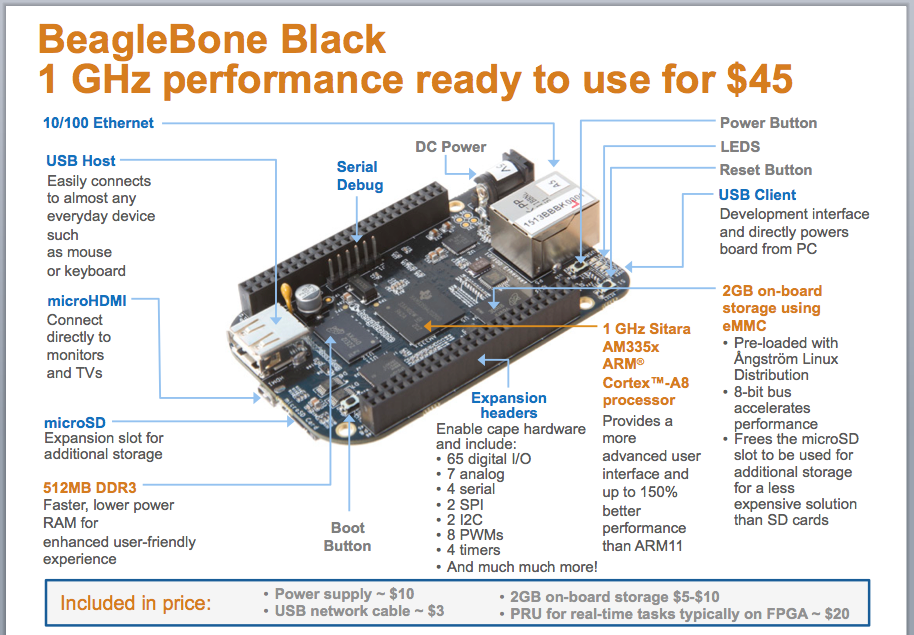
\includegraphics[width=\textwidth]{figures/beagleboneblack-specs}
	\caption{BeagleBone Black開發板}
	\caption*{來源:codeduino.com}
	\label{f:beagleboneblack-specs}
\end{figure}

\section{感測元件}
\subsection{位置姿態感測器}
位置姿態感測器使用Xsens公司所生產的MTi-G整合式感測器,它結合了GPS、加速度計、角速度計、磁力計與壓力計,並內建DSP處理器即時利用Xsens卡爾曼濾波器(Xsens Kalman Filter)
來增進量測的準確度,比起傳統的GPS和姿態航向參考系統(Attitude and Heading Reference System,AHRS)更能提供穩定且低干擾的量測結果,外觀如圖~\ref{f:MTi-G}所示。
其於特定條件下的性能如表~\ref{t:mti-g_performance}所示,請參考使用手冊\cite{Xsens:2012:MTiG_Manual}。

\begin{table}[h!]
	\centering
	\caption{MTi-G Performance Specification}
	\label{t:mti-g_performance}
	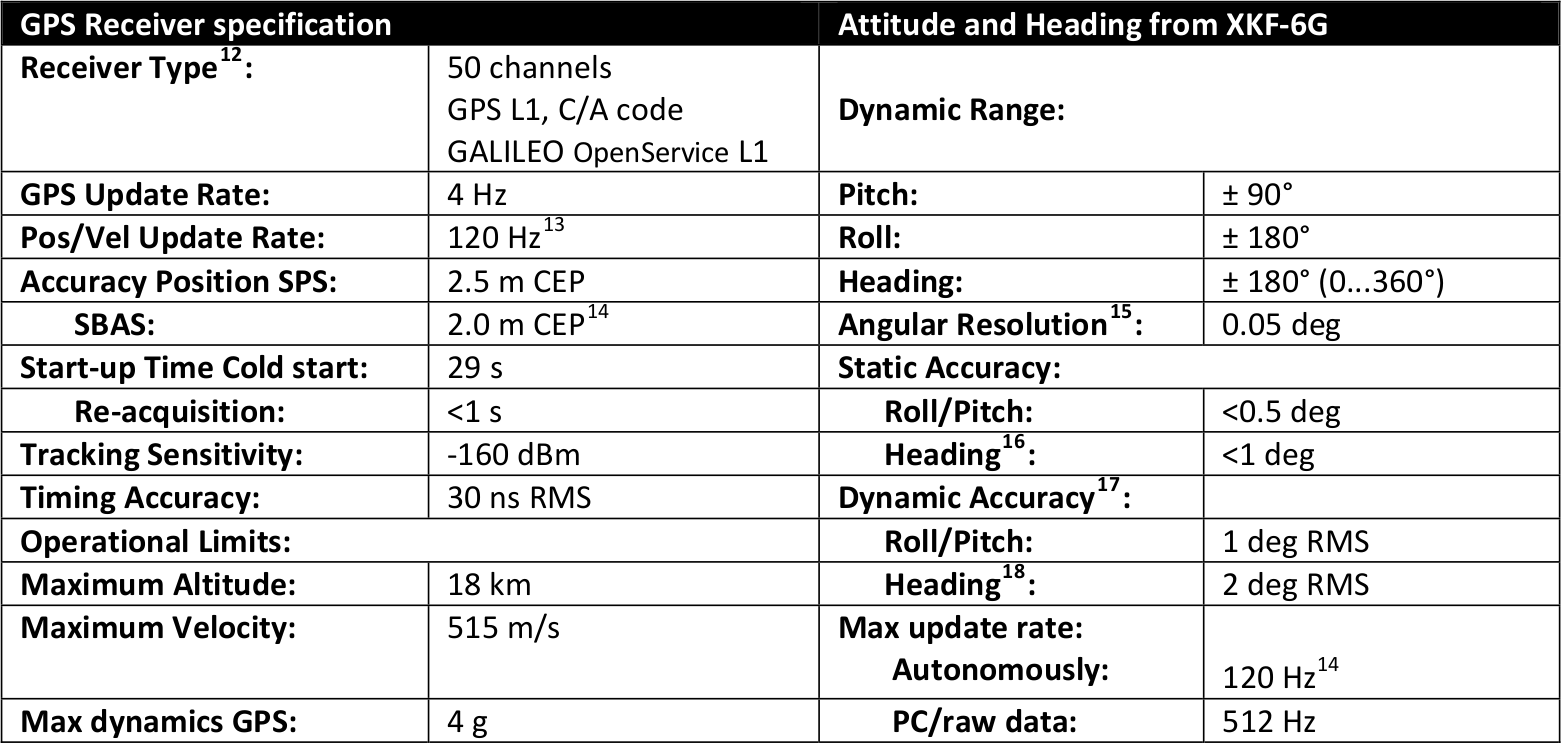
\includegraphics[width=\textwidth]{tables/MTi-G_Performance}
	\caption*{來源:MTi-G User Manual and Technical Documentation\cite{Xsens:2012:MTiG_Manual}}
\end{table}

\begin{figure}[h!]
	\centering
	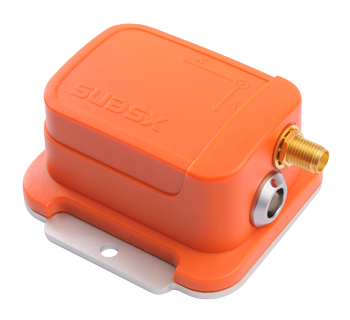
\includegraphics[width=4cm]{figures/MTi-G}
	\caption{Xsens MTi-G AHRS位置姿態感測器}
	\caption*{來源:www.xsens.com}
	\label{f:MTi-G}
\end{figure}

\subsection{掃描式雷射測距儀}
Yun-Trooper II使用HOKUYO公司所生產的URG-04LX-UG01掃描式雷射測距儀來量測週遭環境的變化,規劃路徑以避開障礙物。
其規格如表~\ref{t:urg-specs}所示,外觀如圖~\ref{f:urg}所示

\begin{table}[h!]
	\centering
	\caption{URG-04LX-UG01規格}
	\label{t:urg-specs}
	\begin{tabular}{| l | c |}
		\hline
		光源 & 半導體雷射($\lambda = 785nm$) \\ \hline
		輸入電壓 & 5V DC $\pm 5\%$(USB Power) \\ \hline
		輸入電流 & 500mA(最大800mA) \\ \hline
		量測距離 & 20mm$\sim$4000mm \\ \hline
		距離解析度 & 1mm \\ \hline
		掃描範圍 & $\pm 120\,^{\circ}$ \\ \hline
		角度解析度 & $0.36\,^{\circ}$ \\ \hline
		取樣頻率 & 10Hz \\
		\hline
	\end{tabular}
\end{table}

\begin{figure}[h!]
	\centering
	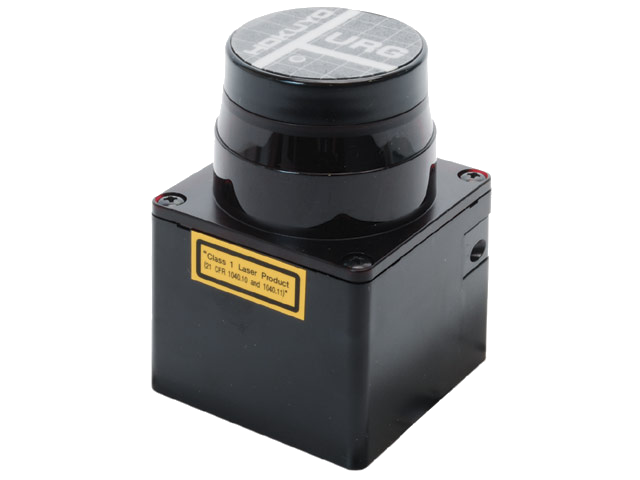
\includegraphics[width=6cm]{figures/URG-04LX-UG01}
	\caption{HOKUYO URG-04LX-UG01掃描式雷射測距儀}
	\caption*{來源:www.hokuyo-aut.jp}
	\label{f:urg}
\end{figure}

\section{驅動元件}

\subsection{轉向伺服機}
為了縮小車輛的迴轉半徑,Yun-Trooper II前後皆具有阿克曼轉向機構(Ackermann Steering Mechanism),
各裝有一顆由Thunder Tiger公司所生產的DS1015數位伺服機做為轉向之動力來源。其規格如表~\ref{t:ds1015-specs}所示,外觀如圖~\ref{f:ds1015}所示。

\begin{table}[h!]
	\centering
	\caption{DS1015數位伺服機規格}
	\label{t:ds1015-specs}
	\begin{tabular}{ | l | c |}
		\hline
		電壓範圍 & 4.8V ~ 6V \\ \hline
		扭力 @ 6V & 14.5kg-cm \\ \hline
		重量 & 66g \\ \hline
		速度 @ 6V & 0.108 sec/$60\,^{\circ}$ \\ \hline
		尺寸(長x寬x高) & 41.8mm x 20.6mm x 39.6mm \\ \hline
		角度範圍 & $180\,^{\circ}$ \\
		\hline
	\end{tabular}
\end{table}

\begin{figure}[h!]
	\centering
	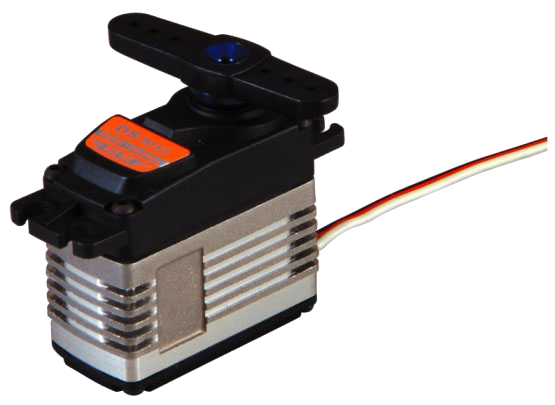
\includegraphics[width=6cm]{figures/DS1015}
	\caption{DS1015數位伺服機}
	\caption*{來源:Thunder Tiger官方網站}
	\label{f:ds1015}
\end{figure}

\subsection{直流馬達}
Yun-Trooper II使用MABUCHI MOTOR公司生產的RS-550VC-7525直流馬達做為車輛之動力來源,其規格如表~\ref{t:rs550vc-specs}所示,外觀如圖~\ref{f:rs550vc}所示。

\begin{table}[h!]
	\centering
	\caption{RS-550VC-7525規格}
	\label{t:rs550vc-specs}
	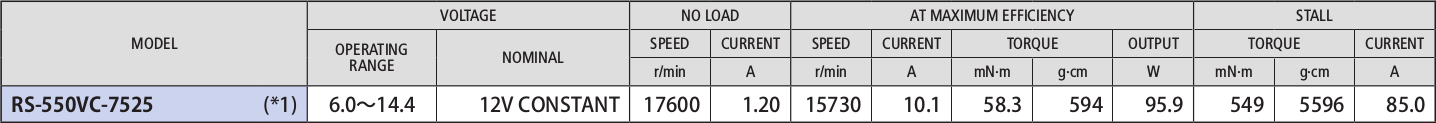
\includegraphics[width=\textwidth]{tables/RS550VC-specs}
	\caption*{來源:MABUCHI MOTOR官方網站}
\end{table}

\begin{figure}[h!]
	\centering
	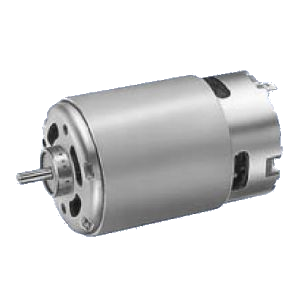
\includegraphics[width=6cm]{figures/motor}
	\caption{RS-550VC-7525直流馬達}
	\caption*{來源:MABUCHI官方網站}
	\label{f:rs550vc}
\end{figure}

\subsection{直流馬達驅動器}
由於BeagleBone Black輸出的PWM訊號為3.3V,最大電流約只有6mA,無法直接驅動直流馬達,
所以使用Pololu公司所生產的MD01B直流馬達驅動器將訊號放大,其外觀如圖~\ref{f:motor_driver}所示。

\begin{figure}[h!]
	\centering
	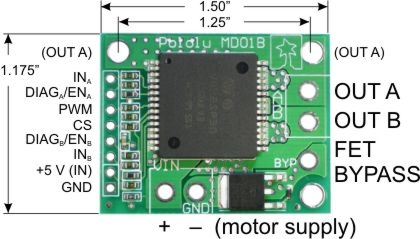
\includegraphics[width=8cm]{figures/motor_driver}
	\caption{Pololu MD01B直流馬達驅動器}
	\caption*{來源:Pololu官方網站}
	\label{f:motor_driver}
\end{figure}

\section{電源供應元件}
Yun-Trooper II使用兩個12V的鋰電池做為電力來源,一顆供應動力系統(直流馬達與伺服機),另一顆供應運算與感測系統(運算核心與感測器)。
其中伺服機需要6.5V的電壓源,運算核心與感測器則需5V電壓源,所以當中使用了兩個飆機器人公司所生產的DC-DC LM2596可調穩壓模組來供應不同的電壓源。
其外觀如圖~\ref{f:lm2596}所示。

\begin{figure}[h!]
	\centering
	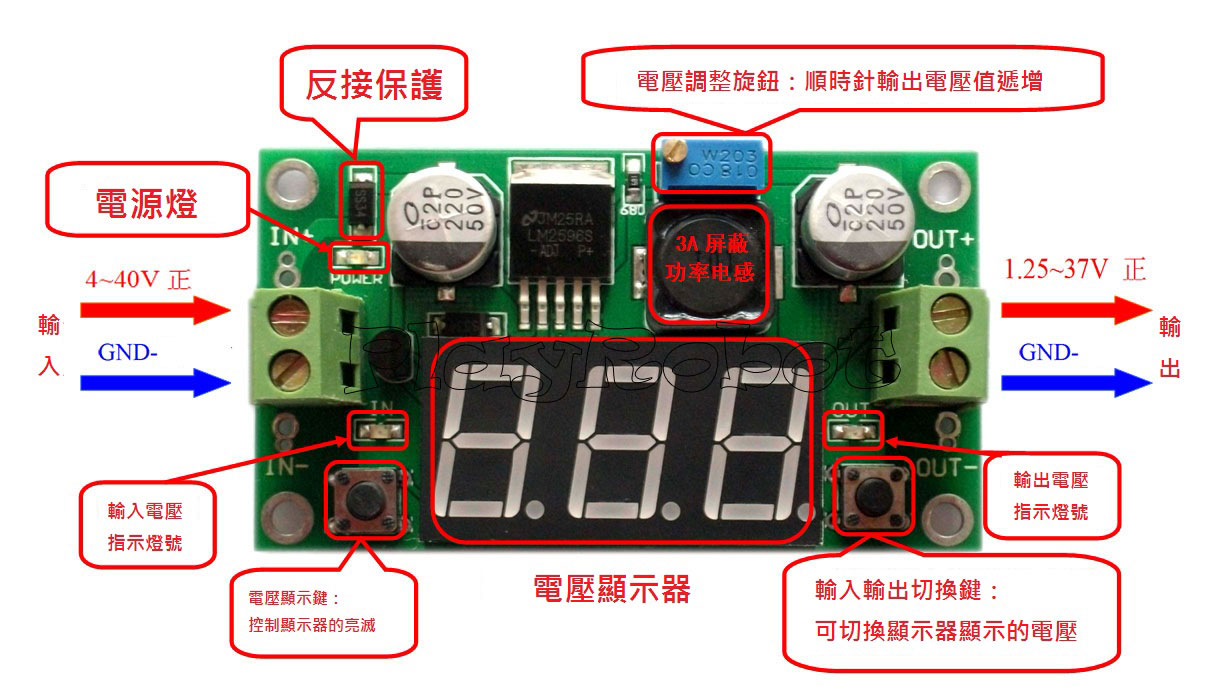
\includegraphics[width=14cm]{figures/LM2596}
	\caption{DC-DC LM2596可調穩壓模組}
	\caption*{來源:飆機器人官方網站}
	\label{f:lm2596}
\end{figure}

\section{通訊元件}
Yun-Trooper II主要是由遠端透過無線通訊控制其功能,其使用Digi International公司所生產的XBee-PRO無線通訊模組做為通訊介面。
XBee-PRO簡單易用,只需在兩端設定相同的鮑率(Baud Rate)即可直接以串列埠(Serial Port)的方式通訊,不需其它設定。
其性能規格如表~\ref{t:xbee_pro}所示,外觀如圖~\ref{f:xbee_pro}所示。
XBee PRO與BeagleBone Black的連接是使用飆機器人公司所生產的XBee轉TTL轉接板,如圖~\ref{f:xbee2ttl}所示;
與個人電腦的連接則是使用同為飆機器人公司所生產的XBee Explorer USB轉接板,如圖~\ref{f:xbee2usb}所示。

\begin{table}[h!]
	\centering
	\caption{XBee PRO無線通訊模組性能規格}
	\label{t:xbee_pro}
	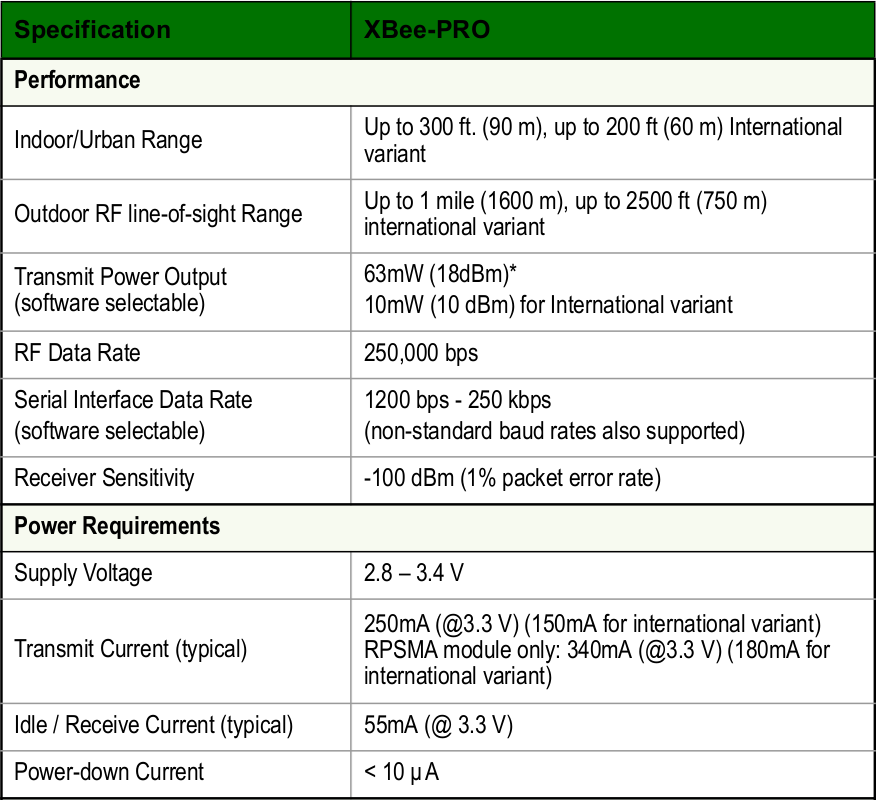
\includegraphics[width=\textwidth]{tables/XBee_PRO}
	\caption*{來源:Digi International官方網站}
\end{table}

\begin{figure}[h!]
	\centering
	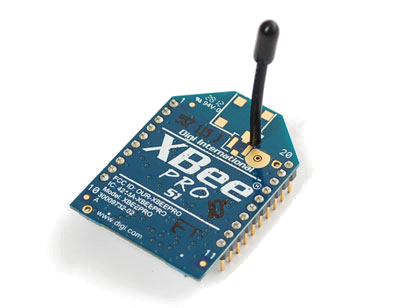
\includegraphics[width=6cm]{figures/xbee_pro}
	\caption{XBee PRO無線通訊模組}
	\caption{來源:digipak.org}
	\label{f:xbee_pro}
\end{figure}

\begin{figure}[h!]
	\centering
	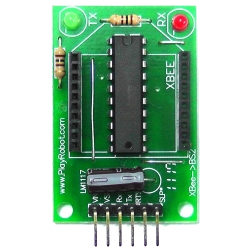
\includegraphics[width=6cm]{figures/xbee2ttl}
	\caption{XBee轉TTL轉接板}
	\caption*{來源:飆機器人官方網站}
	\label{f:xbee2ttl}
\end{figure}

\begin{figure}[h!]
	\centering
	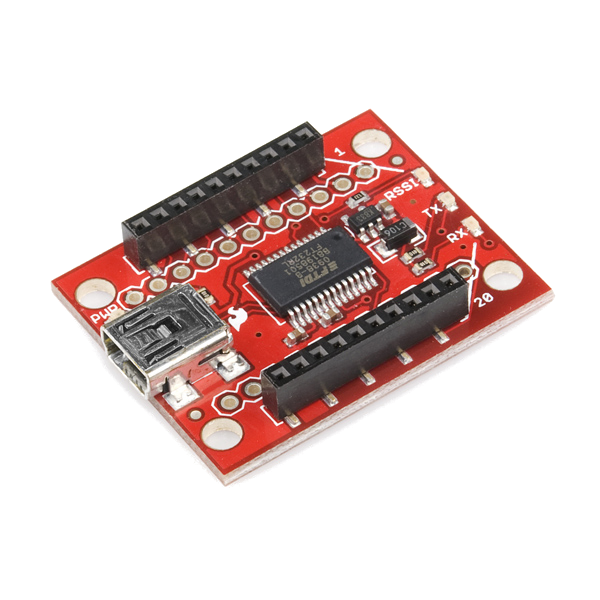
\includegraphics[width=6cm]{figures/xbee2usb}
	\caption{XBee Explorer USB轉接板}
	\caption*{來源:www.sparkfun.com}
	\label{f:xbee2usb}
\end{figure}

